Vuetify jest frameworkiem na licencji MIT  służacym do budowy interfejsów użytkownika w aplikacjach webowych. Projekt ten jest wspierany przez wolontariuszy i sponsorów z całej społeczności Vue. Posiada spójny cykl aktualizacji, oraz możliwość wykupienia wsparcia dla użytku biznesowego. Co tydzień wypuszczany jest również pakiet poprawek złaszanych przez społeczność

Framework ten obsługuje wszystkie główne przeglądarki. Przeglądarki starsze również będą działać jednak wymagają zastosowania pewnych kroków które można bez problemu znaleźć w dokumentacji.

Vuetify dostarcza również swoje płatne rozwiązania takie jak szablony lub też wcześniej wspomniane wsparcie.

Główną zaletą jest łatwność z jaką tworzy się interfejs przy pomocy gotowych komponenetów. Ich mnogość pozwala na tworzenie dowolnych konfiguracji prze potrzeby tworzenia własnych rozwiązań. Dodatkowo dokumentacja jest przejrzysta i intuicyjna. Zarówno osoba początkująca jak i zaawansowana doceni plusy użytkowania owego frameworku.

Jest to obecnie jedno z lepszych rozwiązań na rynku co poświadcza ilość funkcjonalności dostarczanych przez Vuetify (rys. \ref{fig:vuetifyjs})

\begin{figure}[!ht]
    \centering
    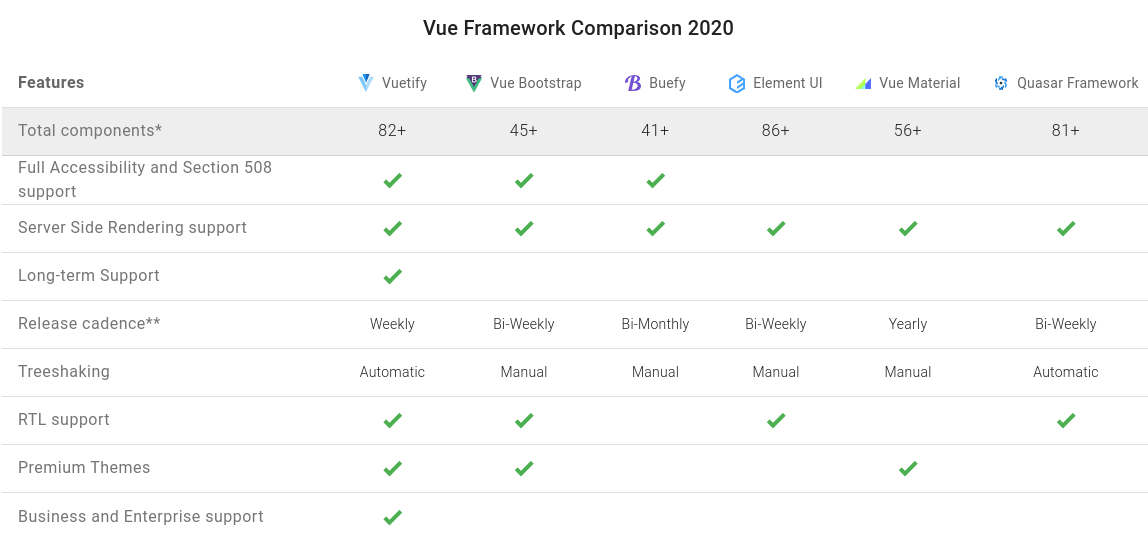
\includegraphics[width=6in]{images/vuetifyjs.png}
    \caption{Porównanie możliwości najbardziej znanych frameworków do Vue \label{fig:vuetifyjs}}
\end{figure}